\chapter{Introducción}

Las vulnerabilidades cuantifican la superficie de ataque digital de un sistema. En particular el stack de componentes expuestos a una red pública o dentro de una red privada compleja incluyen en su versión mínima: firmware, sistema operativo, frameworks varios y múltiples aplicaciones con sus propias arquitecturas. Todos ellos tienen vulnerabilidades conocidas y registradas en bases de datos como CVE\cite{CVE}. Dichas vulnerabilidades constituyen una información útil en la construcción de nuevas aplicaciones de software en la medida en que no se reiteren. Sentido común que no tiene su correlato en la realidad y las vulnerabilidades conocidas se reiteran en nuevos sistemas todo el tiempo.
¿Cómo es posible que esto ocurra? Si bien los modelos de proceso de construcción de software tienen una madurez que aportan técnicas para minimizar el problema, por ejemplo la construcción de modelos de amenazas\cite{Microsoft_Threat_Modeling_Tool}; es frecuente que las herramientas utilizadas y urgencias de entregar funcionalidad conduzcan el desarrollo en la dirección de prácticas que repiten vulnerabilidades conocidas. Más la falta de formación formal en aspectos de ciberseguridad conducen a una escasa conciencia de las consecuencias de repetir fallas conocidas. Cuando se construye software utilizando Content Management Systems (CMS) los 10 principales frameworks representan más del 86\% del market share, con un 65,1\% de WordPress\cite{IONOS_CMS}. Cuando se utiliza este framework, existe una exposición a la historia de sus vulnerabilidades. En la Figura \ref{fig:mi_imagen} se muestra la evolución de la superficie de ataque de los principales CMS del mercado, con año en abscisas y vulnerabilidades descubiertas en ordenadas. Una curva llama la atención, la de WordPress. Sumado a su popularidad no es de extrañar que el escenario conduce a usuarios expuestos.

\begin{figure}[H]
    \centering
    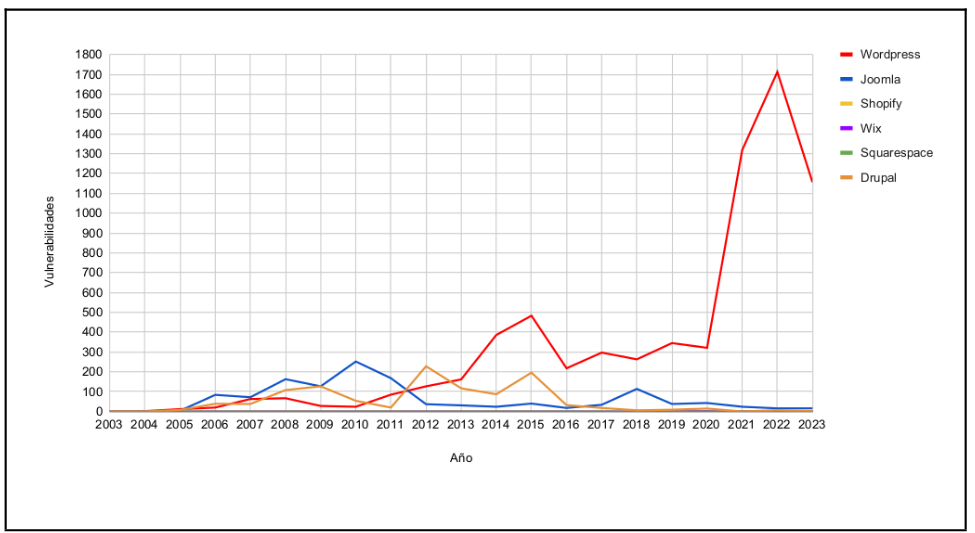
\includegraphics[width=1\textwidth]{Imagenes/wpcms.png}
    \caption{Cantidad de vulnerabilidades de los principales CMS.}
    \label{fig:mi_imagen}
\end{figure}